\section{Characteristics of Annotation Artifacts}
\label{ssec:analysis}

In the previous section we showed that more than half (MultiNLI) or even two thirds (SNLI) of the data can be classified correctly using annotation artifacts.
A possible explanation for the formation and relative consistency of these artifacts is that crowd workers adopt  heuristics in order to generate hypotheses quickly and efficiently.
We identify some of these heuristics by conducting a shallow statistical analysis of the data, focusing on lexical choice (\secref{lexical}) and sentence length (\secref{length}).


\subsection{Lexical Choice} 
\label{ssec:lexical}

To see whether the use of certain words is indicative of the inference class, we compute the point-wise mutual information (PMI) between each word and class in the training set:
\begin{equation*}
\text{PMI} (\textit{word}, \textit{class}) = \log \frac{p(\textit{word}, \textit{class})}{p(\textit{word}, \cdot) p(\cdot, \textit{class})}
\end{equation*}
We apply add-100 smoothing to the raw statistics; 
the aggressive smoothing emphasizes word-class correlations that are highly discriminative. 
Table~\ref{tab:pmi} shows the top words affiliated with each class by PMI, along with the proportion of training sentences in each class containing each word.

Below, we elaborate on the most discriminating words for each NLI class, and suggest possible annotation heuristics that gave rise to these particular artifacts.
However, it is important to note that even the most discriminative words are not very frequent, indicating that the annotation artifacts are diverse, and that crowd workers tend to adopt multiple heuristics for generating new text. 

\begin{table*}[t]
\centering
{
\begin{tabular}{ll} \toprule
\textbf{Premise} & Two dogs are running through a field. \\\midrule
\textbf{Entailment} & There are \textbf{animals} \textbf{outdoors}. \\
\textbf{Neutral} & Some puppies are running \textbf{to catch a stick}. \\
\textbf{Contradiction} & The pets are \textbf{sitting on a couch}. \\\bottomrule
\end{tabular}
}
\caption{The example provided in the annotation guidelines for SNLI. 
Some of the observed artifacts (bold) can be potentially traced back to phenomena in this specific example.}
\label{tab:guidelines}
\end{table*}

\begin{table}
\setlength{\tabcolsep}{2pt}
\centering
\footnotesize{
\begin{tabular}{cllllll}
\toprule
 & \multicolumn{2}{c}{\textbf{Entailment}} & \multicolumn{2}{c}{\textbf{Neutral}} & \multicolumn{2}{c}{\textbf{Contradiction}} \\
\midrule
\multirow{5}{*}{\textbf{SNLI}}       & outdoors & 2.8\%     & tall & 0.7\%          & nobody & 0.1\% \\
                            & least & 0.2\%         & first & 0.6\%         & sleeping & 3.2\% \\
                            & instrument & 0.5\%   & competition & 0.7\%   & no & 1.2\% \\
                            & outside  & 8.0\%     & sad  & 0.5\%         & tv & 0.4\% \\
                            & animal & 0.7\%       & favorite & 0.4\%     & cat  & 1.3\% \\
\midrule
\multirow{5}{*}{\textbf{MNLI}}       & some & 1.6\%           & also & 1.4\%          & never & 5.0\% \\
                            & yes  & 0.1\%         & because & 4.1\%      & no & 7.6\% \\
                            & something & 0.9\%    & popular & 0.7\%      & nothing & 1.4\% \\
                            & sometimes & 0.2\%     & many & 2.2\%          & any & 4.1\% \\
                            & various & 0.1\%       & most & 1.8\%          & none & 0.1\% \\
\bottomrule
\end{tabular}
}
\caption{Top 5 words by $\text{PMI}(\text{\textit{word}}, \text{\textit{class}})$,
along with the proportion of {\it class} training samples  containing {\it word}. MultiNLI is abbreviated to MNLI.}
\label{tab:pmi}
\end{table}


\paragraph{Entailment.}
Entailed hypotheses have generic words such as \textit{animal}, \textit{instrument}, and \textit{outdoors}, which were probably chosen to generalize over more specific premise words such as \textit{dog}, \textit{guitar}, and \textit{beach}.
Other heuristics seem to replace exact numbers with approximates (\textit{some}, \textit{at least}, \textit{various}), and to remove explicit gender (\textit{human} and \textit{person} appear lower down the list).
Some artifacts are specific to the domain, such as \textit{outdoors} and \textit{outside}, which are typical of the personal photo descriptions on which SNLI was built.
Interestingly, the example from the SNLI annotation guidelines (Table~\ref{tab:guidelines}) contains both \textit{animals} and \textit{outdoors}, and also removes the number. 
This example likely primed the annotators, inducing the specific heuristics of replacing \textit{dog} with \textit{animal} and mentions of scenery with \textit{outdoors}.

\paragraph{Neutral.}
Modifiers (\textit{tall}, \textit{sad}, \textit{popular}) and superlatives (\textit{first}, \textit{favorite},\com{ \textit{many},} \textit{most}) are affiliated with the neutral class. 
These modifiers are perhaps a product of a simple strategy for introducing information that is not obviously entailed by the premise, yet plausible. 
Another formulation of neutral hypotheses seems to be through cause and purpose clauses, which increase the prevalence of discourse markers such as \textit{because}. %\com{ and \textit{due}}. 
Once again, we observe that the example from the SNLI annotation guidelines does just that, by adding the purpose clause \textit{to catch a stick} (Table~\ref{tab:guidelines}).

\paragraph{Contradiction.}
Negation words such as \textit{nobody}, \textit{no}, \textit{never} and \textit{nothing} 
are strong indicators of contradiction.\footnote{Similar findings were observed in the ROC story cloze annotation \cite{Schwartz:2017}.}
Other (non-negative) words appear to be part of heuristics for contradicting whatever information is displayed in the premise; \textit{sleeping} contradicts any activity, and \textit{naked} (further down the list) contradicts any description of clothing. 
The high frequency of \textit{cat} probably stems from the many dog images in the original dataset. 
\com{Another seemingly useful strategy replaces any mention of outdoor scenery with some information that implies indoors activity, such as \textit{watching TV} or \textit{sleeping}.}



\subsection{Sentence Length}
\label{ssec:length}

We observe that the number of tokens in generated hypotheses is not distributed equally among the different inference classes. 
Figure~\ref{fig:length} shows that, in SNLI, neutral hypotheses tend to be long, while entailed ones are generally shorter. 
The median length of a neutral hypothesis is 9, whereas 60\% of entailments have 7 tokens or less. 
We also observe that half of hypotheses with at least 12 tokens are neutral, while a similar portion of hypotheses of length 5 and under are entailments, making hypothesis length an effective feature. 
Length is also a discriminatory feature in MultiNLI, but is less significant, possibly due to the introduction of diverse genres.

The bias in sentence length may suggest that crowd workers created many entailed hypotheses by simply removing words from the premise. Indeed, when representing each sentence as a bag of words, 8.8\% of entailed hypotheses in SNLI are fully contained within their premise, while only 0.2\% of neutrals and contradictions exhibit the same property. MultiNLI showed similar trends.



\begin{figure}[t]
\centering
% \subcaptionbox{SNLI}{
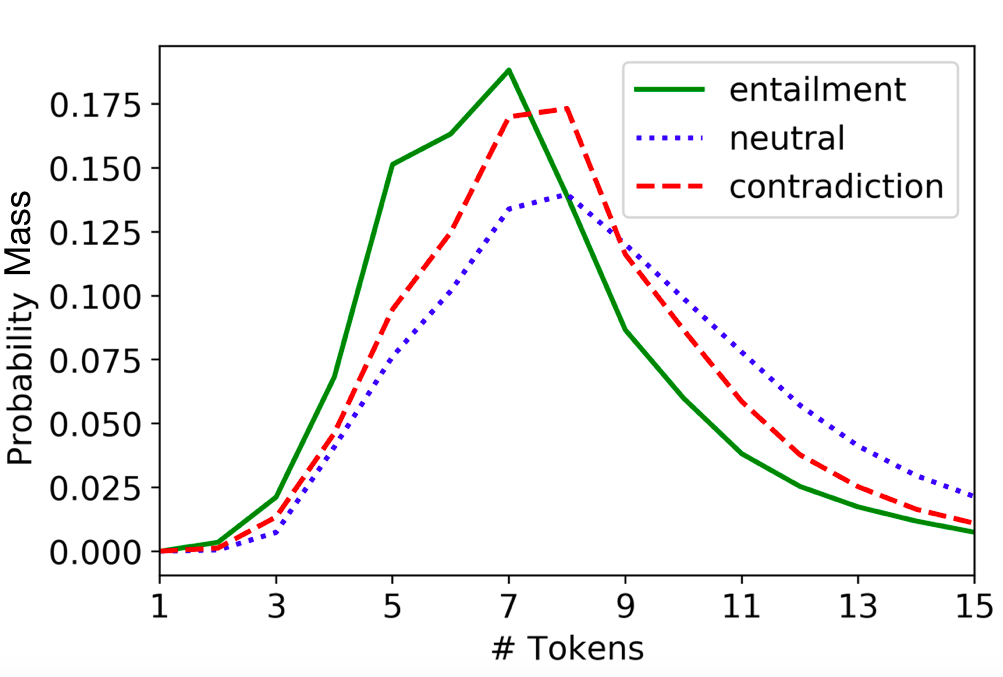
\includegraphics[width=\columnwidth]{fig/snli_length.png}
% }
\caption{The probability mass function of the hypothesis length in SNLI, by class.}

\label{fig:length}
\end{figure}


